\documentclass[11pt]{article}

\usepackage[margin=1in]{geometry}
\usepackage{booktabs}
\usepackage{array}
\usepackage{graphicx}
\usepackage[hidelinks]{hyperref}

\setlength{\emergencystretch}{2em}

% Compile from report/ with:
% latexmk -pdf -interaction=nonstopmode -halt-on-error mi_complication_project.tex

\title{Admission-Time Prediction of Myocardial Infarction Relapse}
\author{Data Analytics Project Report}
\date{\today}

\begin{document}
\maketitle

\begin{abstract}
Predicting relapse at hospital admission for myocardial infarction would allow
earlier preventive care, but admission-time information is limited. On 1700 UCI
records (159 relapses, 9.35\%) we compare three course-approved classifiers
under a leakage-safe protocol: preprocessing is fitted fold-locally, the
threshold is locked on validation, and a single linear SVC is evaluated once on
held-out test data. It detects 8 of 32 relapses at the cost of 62 false alarms
(balanced accuracy \texttt{0.5244}, ROC-AUC \texttt{0.5597}). The contribution
is methodological: an honest, fully auditable baseline showing how weak the
admission-time signal is, rather than an inflated score.
\end{abstract}

\section{Dataset description}

The dataset contains \texttt{1700} hospital records and \texttt{124} columns
\cite{uci-dataset}. The analysis predicts relapse of myocardial infarction
(\texttt{REC\_IM}, column \texttt{122}) from information available at admission. The
target contains \texttt{1541} non-relapse and \texttt{159} relapse observations, or
\texttt{90.65\%} and \texttt{9.35\%}, respectively.

The admission-time feature window follows the dataset specification: input columns
2--112 are eligible except columns \texttt{93}, \texttt{94}, \texttt{95}, and
100--105. The identifier and all eleven non-target outcome columns are also
excluded. The resulting raw candidate matrix contains \texttt{102} predictors. The
complete decision record appears in
\path{report/tables/admission_exclusion_audit.csv}.

\section{Data cleaning}

The raw ``?'' markers are loaded as missing values. Before any learned cleaning,
the admission-safe matrix is split into \texttt{1360} development and \texttt{340} test
rows with stratification and \path{random_state=42}. The development partition is then
split into \texttt{1020} fit and \texttt{340} validation rows.

Within cross-validation, every model/parameter/fold evaluation learns missingness
selection, imputation, clipping, and scaling only from its subfold training rows. The
subfold validation rows are transformed without recalculation. After CV selection, one
final preprocessor is fitted on the \texttt{1020} fit rows and reused unchanged for
validation and test. It removes five predictors above the \texttt{40\%} missingness
threshold: \path{KFK_BLOOD} (\texttt{99.90\%}), \path{IBS_NASL}
(\texttt{96.27\%}), \path{D_AD_KBRIG} and \path{S_AD_KBRIG} (both
\texttt{63.53\%}), and \path{NOT_NA_KB} (\texttt{40.39\%}). Low-cardinality
predictors receive fit-derived mode imputation; other predictors receive fit-derived
median imputation. Fit, validation, and test therefore share the same \texttt{97}
predictors and contain no missing values after transformation.

Continuous predictors are clipped to fit-derived
$[\mu-3\sigma,\mu+3\sigma]$ bounds without dropping observations
\cite{manno-stats}. The learned fill values and clipping bounds are recorded in
\path{report/tables/feature_handling.csv} and
\path{report/tables/sigma_clipping_summary.csv}. No missingness rule, imputation value,
clipping bound, or scaling parameter is fitted on validation or test data.

\section{Exploratory analysis}

All target-linked exploratory analysis is restricted to fit data so that validation and
test labels cannot influence analytical choices. Figure~\ref{fig:class-balance} illustrates
why plain accuracy is not an adequate primary criterion. Figure~\ref{fig:missingness}
reports missingness in the same fit partition.

\begin{figure}[htbp]
\centering
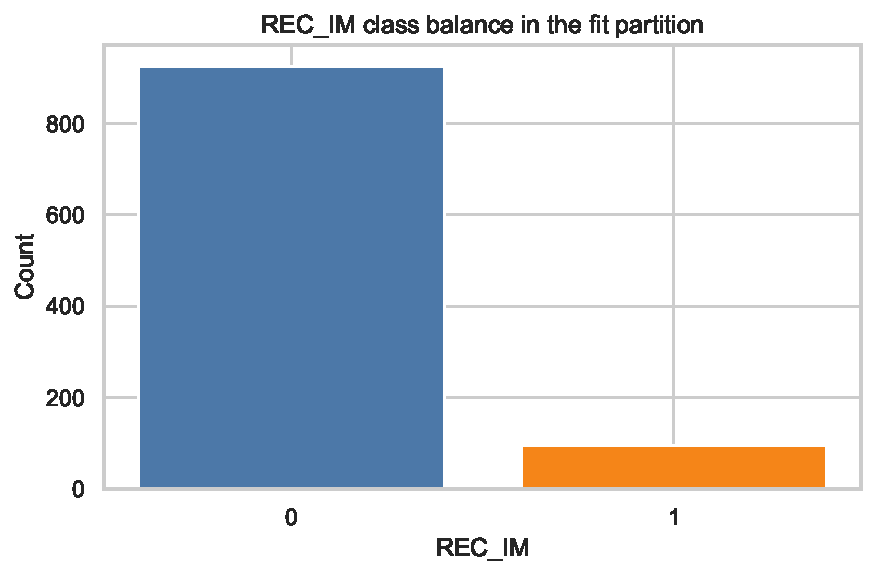
\includegraphics[width=0.62\textwidth]{figures/class_balance}
\caption{Fit-partition distribution of \texttt{REC\_IM}: 925 non-relapse and 95
relapse cases.}
\label{fig:class-balance}
\end{figure}

\begin{figure}[htbp]
\centering
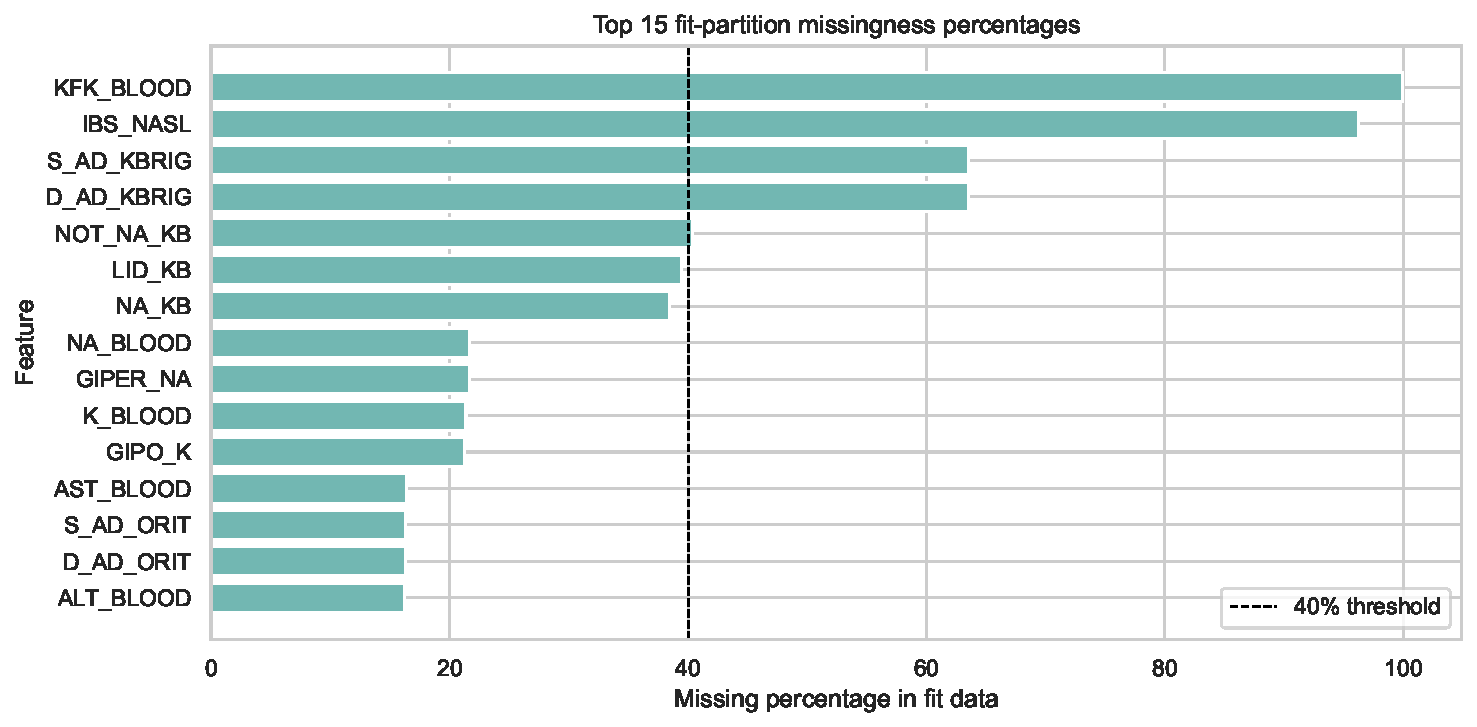
\includegraphics[width=0.92\textwidth]{figures/missingness_top15}
\caption{Top-15 missingness percentages in the fit partition. The dashed line marks the
40\% removal threshold; five predictors exceed it.}
\label{fig:missingness}
\end{figure}

The strongest simple correlation with the target is \texttt{zab\_leg\_02}
(\texttt{0.1184}), followed by \texttt{AGE} (\texttt{0.1057}),
\texttt{STENOK\_AN} (\texttt{0.0979}), and \texttt{np\_01} (\texttt{0.0978}). Their
small magnitudes suggest weak marginal signal. The complete values are exported in
\path{report/tables/top_correlations.csv}; Figures~\ref{fig:distributions} and
\ref{fig:heatmap} provide the corresponding descriptive views.

\begin{figure}[htbp]
\centering
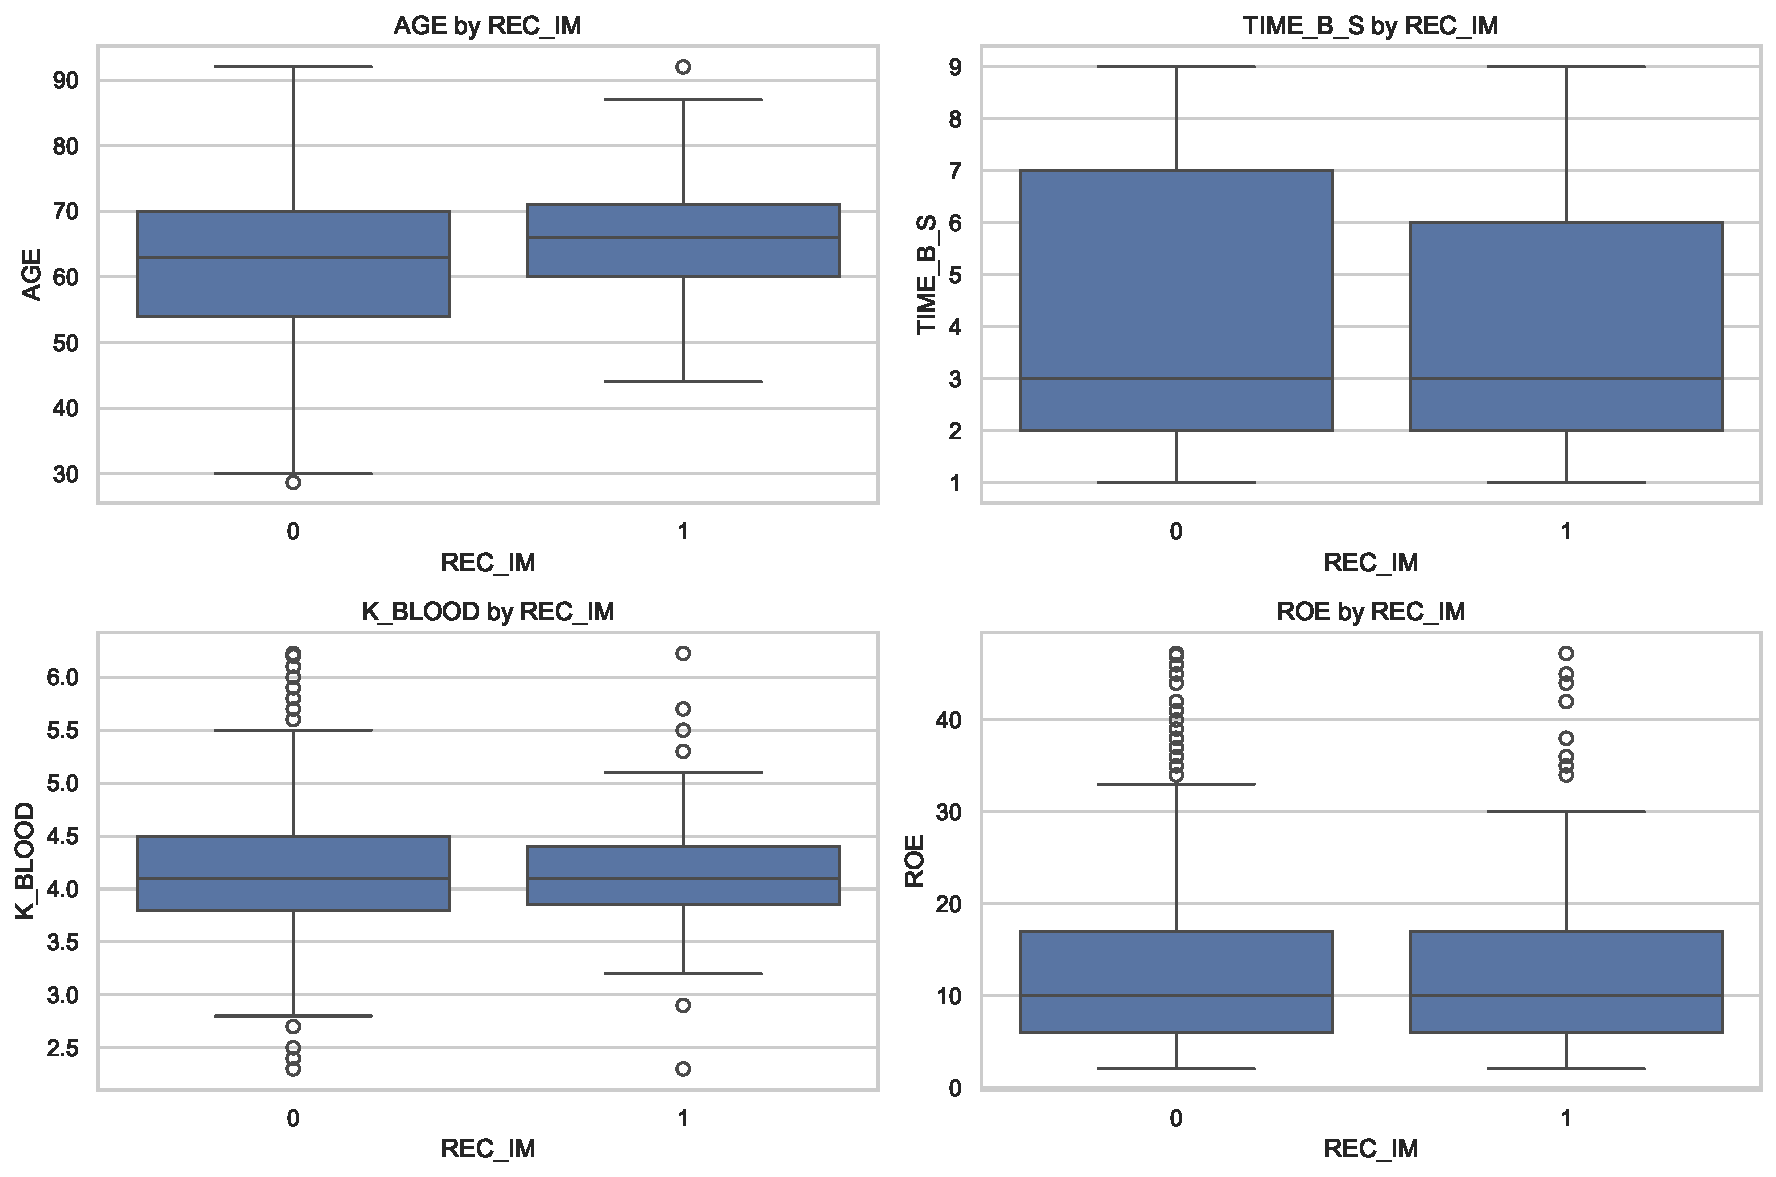
\includegraphics[width=\textwidth]{figures/key_distributions}
\caption{Selected admission-time predictor distributions by \texttt{REC\_IM} class.}
\label{fig:distributions}
\end{figure}

\begin{figure}[htbp]
\centering
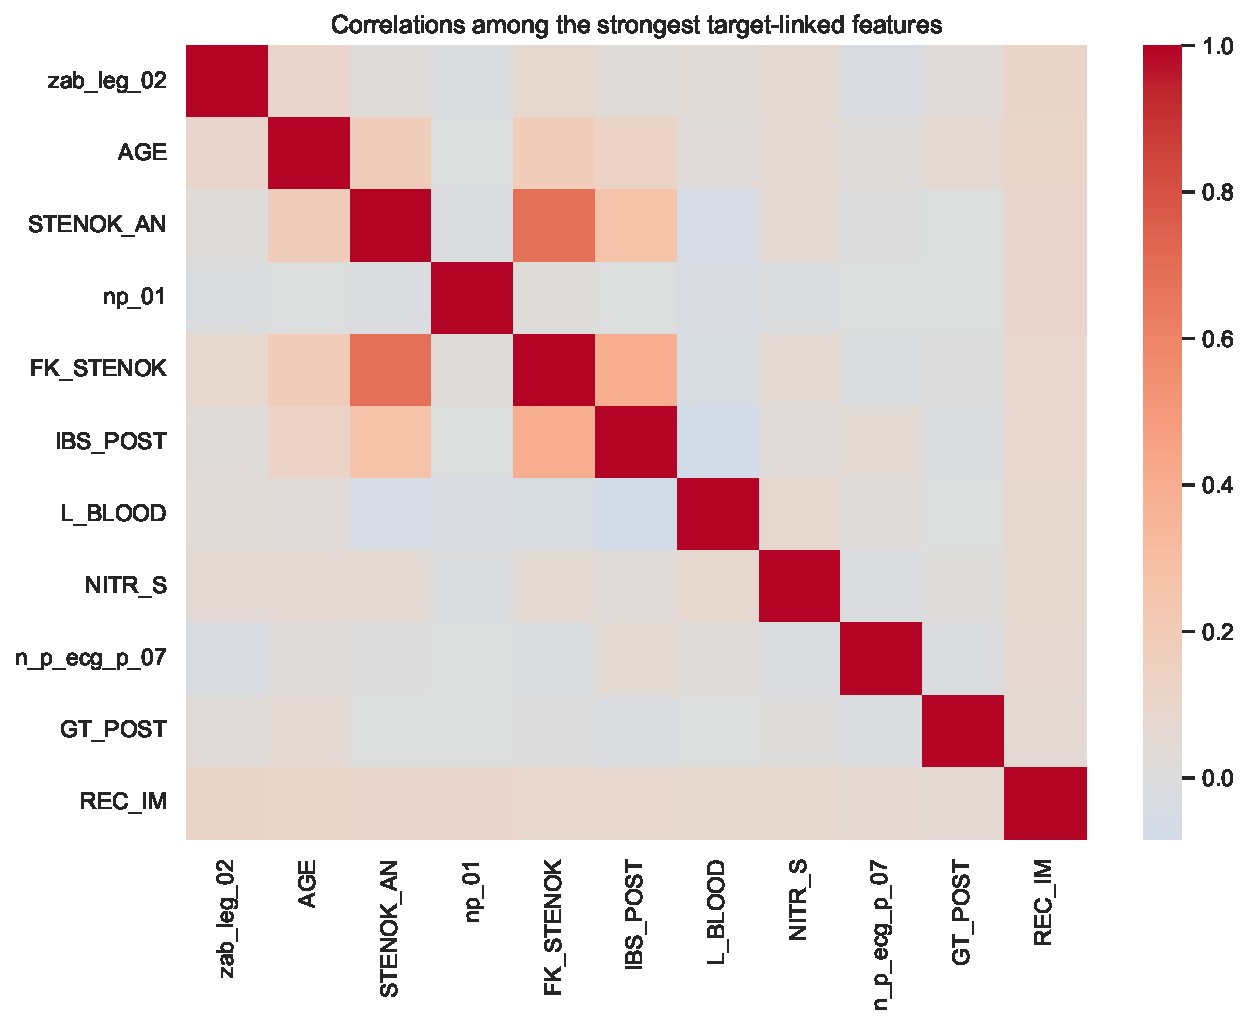
\includegraphics[width=0.82\textwidth]{figures/correlation_heatmap}
\caption{Correlation matrix for the strongest target-linked predictors and
\texttt{REC\_IM}.}
\label{fig:heatmap}
\end{figure}

\subsection{Unsupervised exploration}

K-means is fitted to the scaled descriptive feature matrix for exploratory phenotyping.
The silhouette criterion selects $K=2$ with score \texttt{0.2599}. The fit-partition
clusters contain \texttt{104} and \texttt{916} observations, with relapse rates
\texttt{5.8\%} and \texttt{9.7\%}. Figure~\ref{fig:silhouette} reports the full sweep.

\begin{figure}[htbp]
\centering
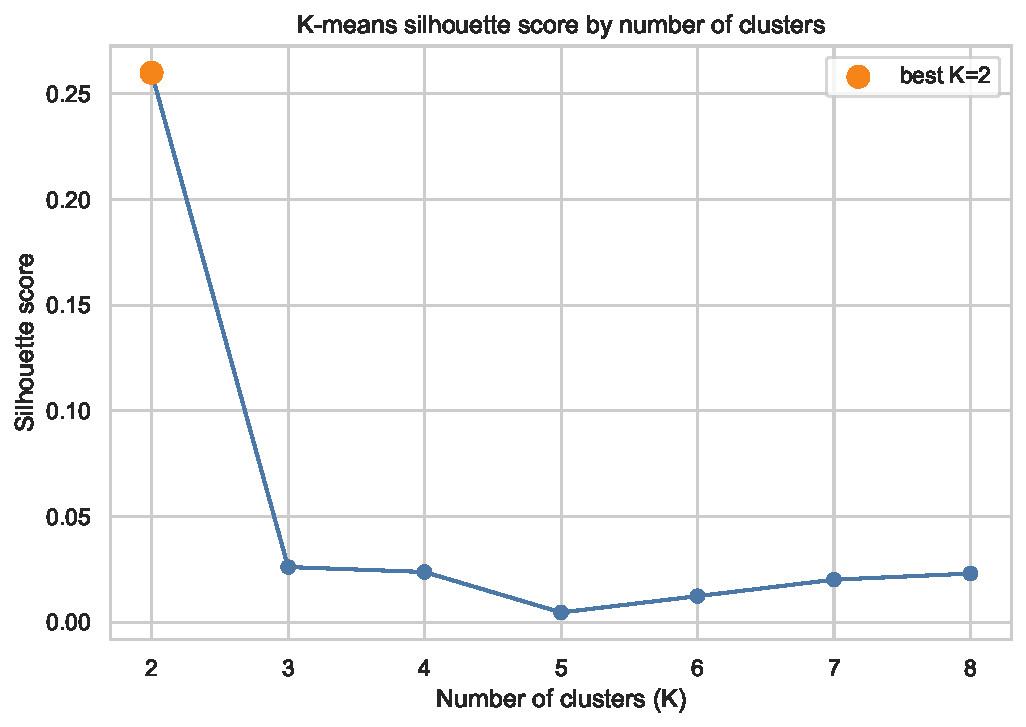
\includegraphics[width=0.72\textwidth]{figures/silhouette_scores}
\caption{Silhouette score for $K\in\{2,\ldots,8\}$; the marked maximum selects $K=2$.}
\label{fig:silhouette}
\end{figure}

PCA is fitted only to display these clusters in two dimensions
\cite{manno-multivariate}. It is not used to transform predictors for logistic
regression, the decision tree, or SVC.

\begin{figure}[htbp]
\centering
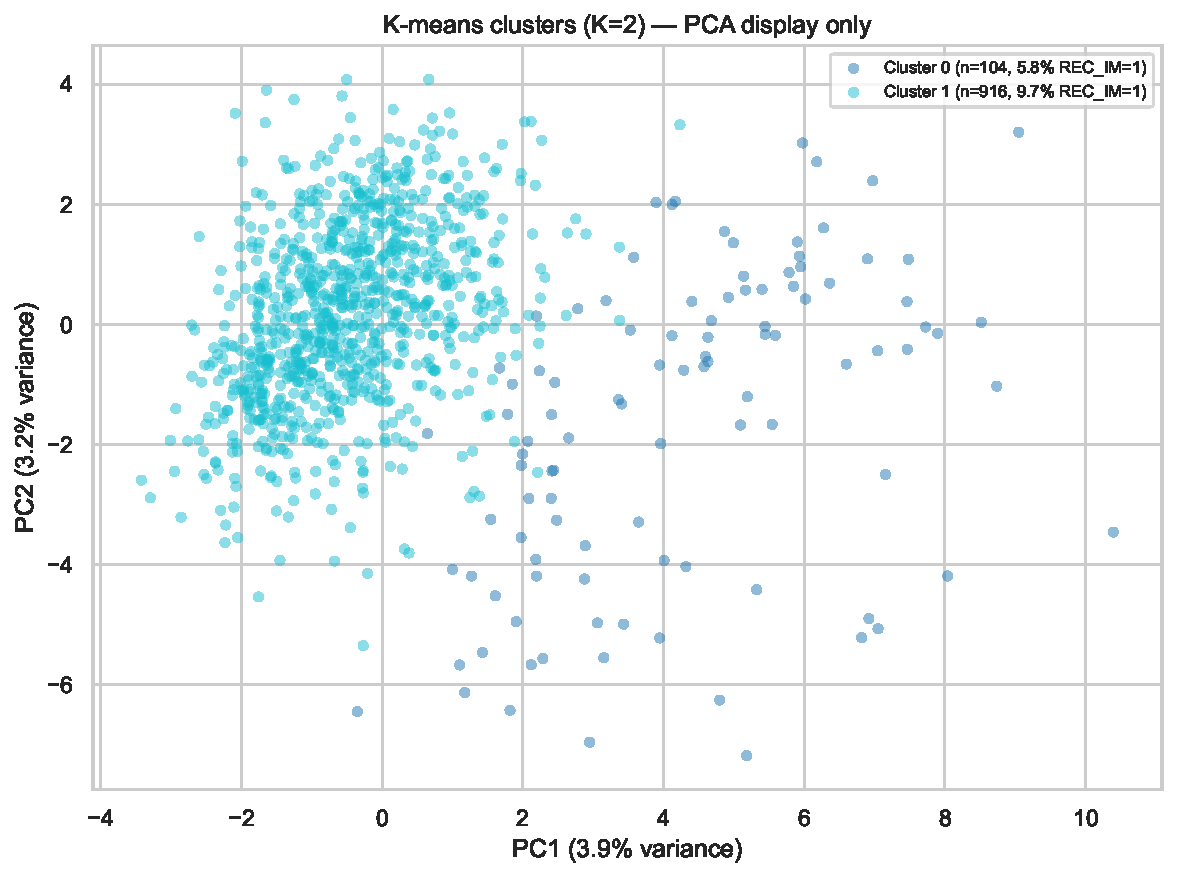
\includegraphics[width=0.82\textwidth]{figures/cluster_pca}
\caption{Two-dimensional PCA display of the fitted K-means clusters. PCA is used only
for this visualisation and is not part of supervised modeling.}
\label{fig:cluster-pca}
\end{figure}

\section{Main analysis: objective and methods adopted}

Logistic regression, an entropy decision tree, and SVC are compared using manual,
deterministic, stratified five-fold cross-validation on the raw fit partition
\cite{manno-supervised}. For each model/parameter/fold evaluation, preprocessing and
optional standardisation are fitted on \texttt{816} subfold training rows and applied
unchanged to \texttt{204} subfold validation rows. The criterion declared before test
evaluation is highest mean fold balanced accuracy; lower fold standard deviation and
then the parameter signature break ties. Table~\ref{tab:cv} shows that this rule
preselects the linear SVC. Test metrics do not enter this decision.

\begin{table}[htbp]
\centering
\small
\setlength{\tabcolsep}{4pt}
\begin{tabular}{lrrl}
\toprule
Model & CV bal. acc. & CV std. & Selected hyperparameters \\
\midrule
SVC & 0.6253 & 0.0437 & \texttt{C=0.1; balanced; linear} \\
Logistic regression & 0.6176 & 0.0545 & \texttt{C=0.1; balanced} \\
Decision tree & 0.5575 & 0.0691 & \texttt{alpha=0.01; balanced; leaf=1} \\
\bottomrule
\end{tabular}
\caption{Model-family and hyperparameter selection on the fit partition.}
\label{tab:cv}
\end{table}

The weighted-minus-unweighted CV balanced-accuracy differences are \texttt{0.1228} for
SVC, \texttt{0.0943} for logistic regression, and \texttt{0.0385} for the tree. The
full comparisons are in \path{report/tables/baseline_vs_weighted.csv}. Tree pruning is
shown in Figure~\ref{fig:pruning}.

\begin{figure}[htbp]
\centering
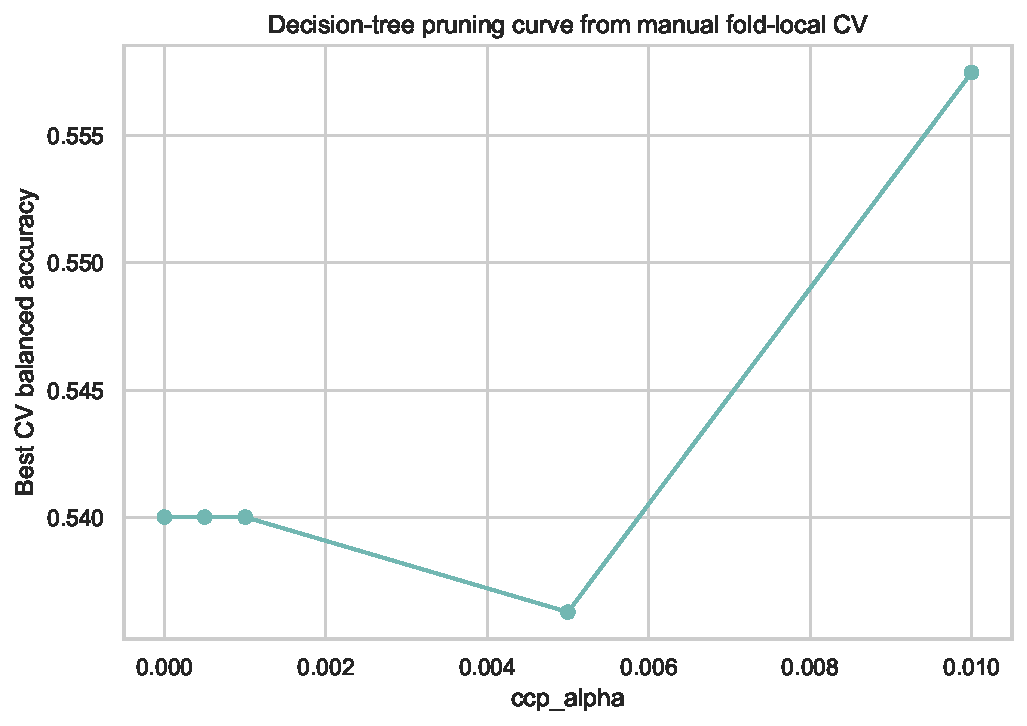
\includegraphics[width=0.72\textwidth]{figures/tree_pruning_curve}
\caption{Best decision-tree CV balanced accuracy at each searched
\texttt{ccp\_alpha}.}
\label{fig:pruning}
\end{figure}

Only the CV winner is evaluated on validation. Its threshold is selected by balanced
accuracy, followed by recall, precision, F1, and proximity to the default threshold.
The selected SVC threshold is \texttt{0.5056}; validation balanced accuracy is
\texttt{0.6246}, recall \texttt{0.4375}, precision \texttt{0.1944}, and F1
\texttt{0.2692}. Figure~\ref{fig:threshold} therefore shows exactly one model.

\begin{figure}[htbp]
\centering
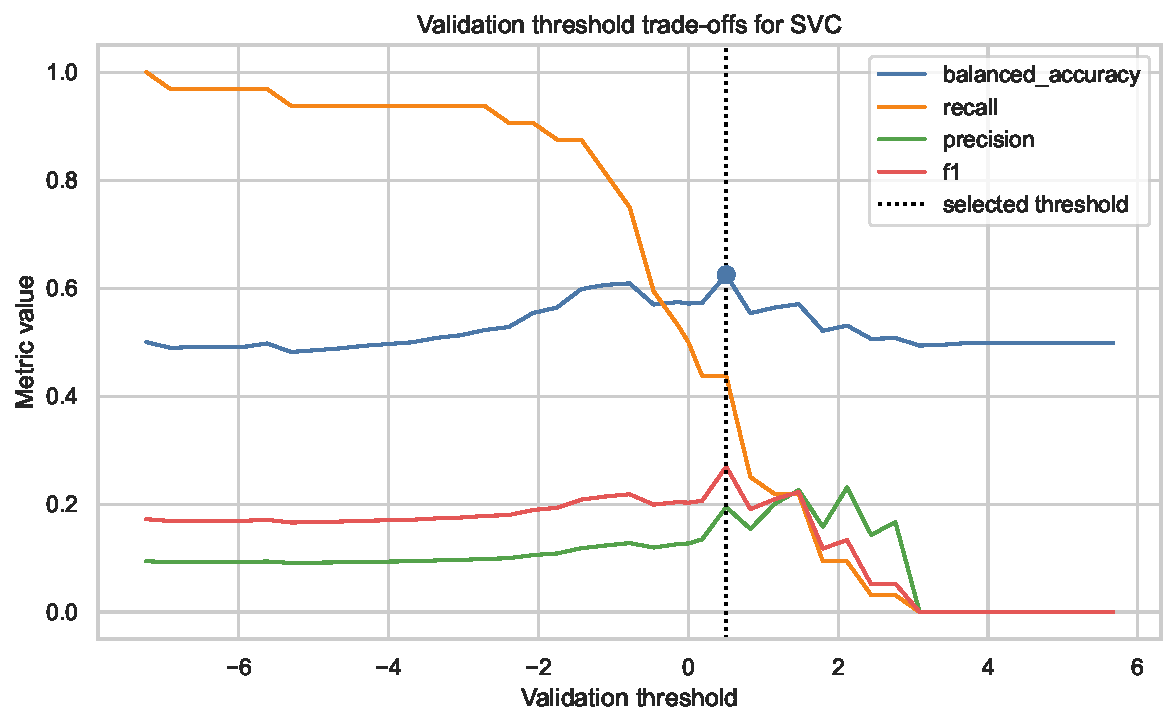
\includegraphics[width=0.88\textwidth]{figures/threshold_tradeoffs}
\caption{Validation threshold sweep for the CV-preselected SVC. Competing families are
not evaluated on validation; the threshold is selected from the same fitted model that
is later evaluated on test.}
\label{fig:threshold}
\end{figure}

After selection, one preprocessor, scaler, and linear SVC are fitted on the fit partition
only. Validation is transformed by these objects to choose the threshold, and no refit
follows. Test is then transformed by the same objects and evaluated once. The per-fold
evidence is exported in \path{report/tables/cv_fold_preprocessing_audit.csv}; the outer
stage record is exported in \path{report/tables/evaluation_protocol.csv}.

\section{Preview/summary of results}

The preselected SVC is the only model evaluated on test. At threshold
\texttt{0.5056}, it obtains accuracy \texttt{0.7471}, balanced accuracy
\texttt{0.5244}, recall \texttt{0.2500}, precision \texttt{0.1143}, F1
\texttt{0.1569}, and ROC-AUC \texttt{0.5597}. The operating point detects 8 of 32
relapse cases and generates 62 false positives. No test-set ranking of model families
is performed.

\section{Detailed results}

\begin{table}[htbp]
\centering
\small
\begin{tabular}{lrrrrrr}
\toprule
Model & Accuracy & Bal. acc. & Recall & Precision & F1 & ROC-AUC \\
\midrule
SVC & 0.7471 & 0.5244 & 0.2500 & 0.1143 & 0.1569 & 0.5597 \\
\bottomrule
\end{tabular}
\caption{The single final evaluation on the isolated test partition.}
\label{tab:test}
\end{table}

The test confusion counts are TN $=246$, FP $=62$, FN $=24$, and TP $=8$.
Figure~\ref{fig:roc} uses the same continuous SVC scores as Table~\ref{tab:test}; it
does not include unselected model families.

\begin{figure}[htbp]
\centering
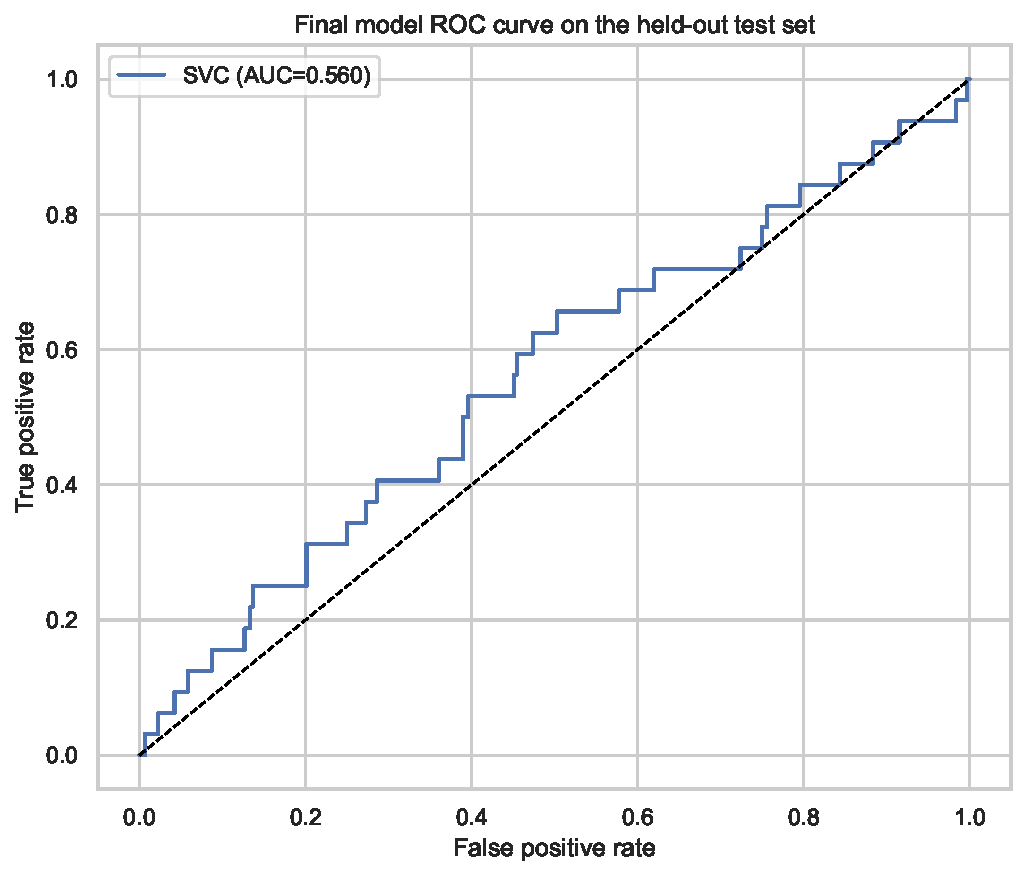
\includegraphics[width=0.78\textwidth]{figures/roc_curves}
\caption{ROC curve for the preselected final SVC on the held-out test set.}
\label{fig:roc}
\end{figure}

Balanced accuracy modestly exceeds chance, while precision remains low because the
selected operating point favours relapse sensitivity in an imbalanced sample. The
ROC-AUC of \texttt{0.5597} similarly indicates weak ranking discrimination. These
values are descriptive estimates for the fixed analysis and do not constitute clinical
validation.

\section{Conclusions}

The analysis preserves the admission-time information boundary and completely isolates
test data from model-family, hyperparameter, and threshold selection. Every CV fold fits
preprocessing and scaling on subfold training rows only. The predeclared criterion
selects a linear SVC; one fit-only preprocessor, scaler, and SVC are then reused for
validation threshold selection and a single test evaluation without refitting. The
resulting balanced accuracy of \texttt{0.5244} and ROC-AUC of \texttt{0.5597} show that
the evaluated admission variables provide only limited signal for \texttt{REC\_IM}.
PCA contributes only a two-dimensional cluster display and does not alter the supervised
predictors. Validation is intentionally excluded from final fitting so that its sole
supervised role remains threshold selection.

\begin{thebibliography}{9}

\bibitem{uci-dataset}
S.~E.~Golovenkin, V.~A.~Shulman, D.~A.~Rossiev, P.~A.~Shesternya,
S.~Yu.~Nikulina, Yu.~V.~Orlova, and V.~F.~Voino-Yasenetsky,
\emph{Myocardial Infarction Complications},
UCI Machine Learning Repository, 2020.
doi: \href{https://doi.org/10.24432/C53P5M}{10.24432/C53P5M}.

\bibitem{manno-supervised}
A.~Manno,
\emph{Data Analytics (and Data Driven Decision): Supervised Learning},
Department of Information Engineering, Computer Science and Mathematics,
University of L'Aquila, academic year 2025--2026.

\bibitem{manno-stats}
A.~Manno,
\emph{Data Analytics (and Data Driven Decision): Basic Statistics},
Department of Information Engineering, Computer Science and Mathematics,
University of L'Aquila, academic year 2025--2026.

\bibitem{manno-multivariate}
A.~Manno,
\emph{Data Analytics (and Data Driven Decision): Multivariate Statistics and Principal
Component Analysis},
Department of Information Engineering, Computer Science and Mathematics,
University of L'Aquila, academic year 2025--2026.

\end{thebibliography}

\end{document}
